\documentclass[oneside]{article}
\usepackage[total={18cm, 21cm}, top=2cm, left=2cm]{geometry}
\parindent = 0mm % sin sangría
\usepackage{latexsym, amsmath, amssymb, amsfonts}
\usepackage[utf8]{inputenc}
\usepackage{graphicx}
\usepackage[spanish]{babel}
\usepackage{float}
\usepackage{longtable, multirow, booktabs}
\usepackage{caption}
\usepackage{makecell}
\usepackage{hyperref}
\usepackage{listings}

\title{Bitacora - Domótica}
\author{
Julio Rubén Sanic Martínez 2012-2228\\
Alejandro Camey Mendez 201503792
}

\begin{document}
\maketitle

\section*{Semana 22-26 de Agosto}
\begin{itemize}
\item \textbf{Problema:} Dar confort y seguridad en los hogares por medio del IOT.
\item \textbf{Alcances:} 
\begin{itemize}
\item Comunicación inalámbrica
\item Control mediante una interfaz gráfica
\item Envoltorio del dispositivo a base de plástico
\item Autonomía con baterías
\item Programación de temporizadores y alarmas
\item Registro de actividades
\end{itemize} 
\item \textbf{Solución:}
Se pretende dar solución al problema mediante los dispositivos ESP8266 y ESP32, que contienen WiFi y un stack TCP/IP completo. Programados mediante Arduino o MicroPython, utilizando el protocolo de red M.Q.T.T. (Message Queuing Telemetry Transport).
\\
La cubierta se pretende que sea de plástico, por tanto, la impresión 3D es imprescindible. Y, para la interfaz gráfica se planean soluciones mediante el uso de Python y JavaScript.
\end{itemize}
\textbf{\Large Pilares}
\begin{itemize}
\item \textbf{Recursos humanos virtuales:}
\begin{itemize}
\item Impresión 3D en terceros.
\item Fabricación de placas electrónicas por medio de terceros.
\end{itemize}
\item \textbf{Activos Ajenos:}
\begin{itemize}
\item Servidores en AWS (Amazon Web Services)
\end{itemize}
\end{itemize}
\newpage

\section*{Semana, 29 de Agosto - 02 de Septiembre}
\subsection*{Inversion del protótipo}

\begin{table}[H]
\centering
\begin{longtable}[c]{llll}
\toprule
Descripción & cantidad & precio unitario (Q) & total (Q) \\
\midrule
\multicolumn{4}{c}{Interruptor}\\
\hline
ESP8266 & 1 & 50 & 50 \\
Batería de litio 1800mAh & 4 & 40 & 160 \\ 
TRIAC MAC97A6 & 2 & 4 & 8 \\
Optoacoplador MOC3021 & 2 & 5 & 10 \\
Resistencia 1/4 W 1k$\Omega$ & 2 & 0.5 & 1 \\
Resistencia 1/4 W 10k$\Omega$ & 1 & 0.5 & 0.5 \\
Resistencia 1/4 W 330$\Omega$ & 1 & 0.5 & 0.5 \\
Capacitor cerámico 104 & 1 & 1 & 1 \\
Pulsador normalmente abierto & 2 & 1 & 2 \\
Sujetador de 4 baterías AA & 1 & 6 & 6 \\
Transformador 12V 1A c/tab & 1 & 62 & 62 \\
\hline
total & & & 301\\
\hline
\multicolumn{4}{c}{Detector de Objetos}\\
\hline
ESP8266 & 1 & 50 & 50 \\
Resistencia 1/4 W 1k$\Omega$ & 1 & 0.5 & 0.5 \\
Resistencia 1/4 W 10k$\Omega$ & 1 & 0.5 & 0.5 \\
Capacitor cerámico 104 & 1 & 1 & 1 \\
Pulsador normalmente abierto & 2 & 1 & 2 \\
Sensor Ultrasónico HC-SR05 & 1 & 25 & 25 \\
\hline
total & & & 79\\
\hline
\multicolumn{4}{c}{Caja de sensores}\\
\hline
ESP32 & 1 & 100 & 100 \\
Sensor de llama & 1 & 16 & 16 \\
Sensor de gas butano MQ-9 & 1 & 34 & 34 \\
Sensor de temperatura LM35 & 1 & 21 & 21 \\
\hline
total & & & 171\\
\hline

FT232R & 1 & 36 & 36 \\
Horas-hombre (electrónica) & 20 & 15 & 300 \\
Horas-hombre (programación) & 80 & 15 & 1200 \\
\hline
TOTAL & & & 2087 \\
\hline
 
\end{longtable}
\caption*{Inversión protótipo}
\end{table}


\subsection*{Inversión Total}
\begin{table}[H]
\centering
\begin{longtable}[c]{llll}
\toprule
Descripción & cantidad & precio unitario (Q) & total (Q) \\  
\midrule

Múltimetro modelo MUT-33 marca TRUPER & 1 & 175 & 175 \\
Múltimetro modelo MUT-830 marca TRUPER & 1 & 100 & 100 \\
Protoboard 830 puntos & 4 & 38 & 152 \\
Fuente de Alimentación 60 W & 1 & 115 & 115 \\
Escritorio & 1 & 600 & 600 \\
Silla & 1 & 200 & 200 \\
Protótipo & & & 2087 \\
\hline
TOTAL & & & 3429\\
\hline 

\end{longtable}
\caption*{Inversión Inicial }
\end{table}

\subsection*{Costos Variables y Costos Fijos}
\begin{table}[H]
\centering

\begin{longtable}[c]{llll}
\toprule
\multicolumn{2}{c}{Costos Fijos} & \multicolumn{2}{c}{Costos Variables} \\
\midrule
Descripción & total & Descripción & total \\
\hline 
Renta Garage & 600 & ESP8266 Interruptor &  166 \\
Renta de Servidor para Broker M.Q.T.T \\+ pago de hosted zones & 50 & ESP8266 Detector & 79  \\
Renta de Servidor para \\ página web y publicidad & 50 & ESP8266 Caja de sensores & 171 \\
Publicidad en Google & 100 & Empaque & 5 \\
Factura de Electricidad & 100 & Envío & 15 \\
Sueldo (Fin de semana) & 1500 & &\\
Amortización inversión a 2 años & 143 & & \\
\hline
TOTAL & 2543 &  TOTAL & 436 \\
\hline
\end{longtable}
\caption*{Costos Variables y Costos Fijos}
\end{table}

\subsection*{Punto de Equilibrio}
Ecuación de punto de equilibrio:
$$Q = \frac{CF}{(P-CV)}$$
Donde:
\begin{itemize}
\item $CF$ son los costos fijos
\item $CV$ son los costos variables
\item $P$ es el precio del producto 
\end{itemize}
Considerando
\begin{itemize}
\item $CF = Q2543$
\item $CV = Q436$
\item $P = CV * 1.5 = Q654$
\end{itemize}
Da como resultado:
$$Q = \frac{2543}{654-436}=11$$
Como conclusión, se tienen que vender 11 juegos de dispositivos para cubrir los gastos y el sueldo. Después de eso, se genera ganancia.

\newpage
\section*{Semana, 05 de septiembre - 09 de Septiembre}
Se realizó un cronógrama de actividades, mostrando el avance en semanas anteriorres y una semana de anticipo.  
\subsection*{Cronógrama de actividades}

\begin{table}[H]
\begin{longtable}[c]{p{5cm} p{9cm}}
\toprule
Fecha & Actividad \\
\midrule
Agosto 22-26 & Definición y Alcances del proyecto \\
\hline
Agosto 29- Septiembre 02 & Punto de Equilibrio \\
\hline
Septiembre 05 - 09 & Pruebas de alimentación (baterías) y configuración inicial del broker Mosquitto en la nube\\
\hline
Septiembre 12 - 16 & Programación inicial en MicroPython/Arduino y análisis de interfaz de usuario \\ 
\hline 
Septiembre 19 - 23 & Programación de sensores y pruebas del broker con un cliente M.Q.T.T \\
\hline

\end{longtable}
\caption*{Cronograma de actividaes}
\end{table}

\subsection*{Configuración del broker Mosquitto}
El alojamiento del broker se realizó en una instancia E2C en AWS:
\begin{figure}[H]
\centering
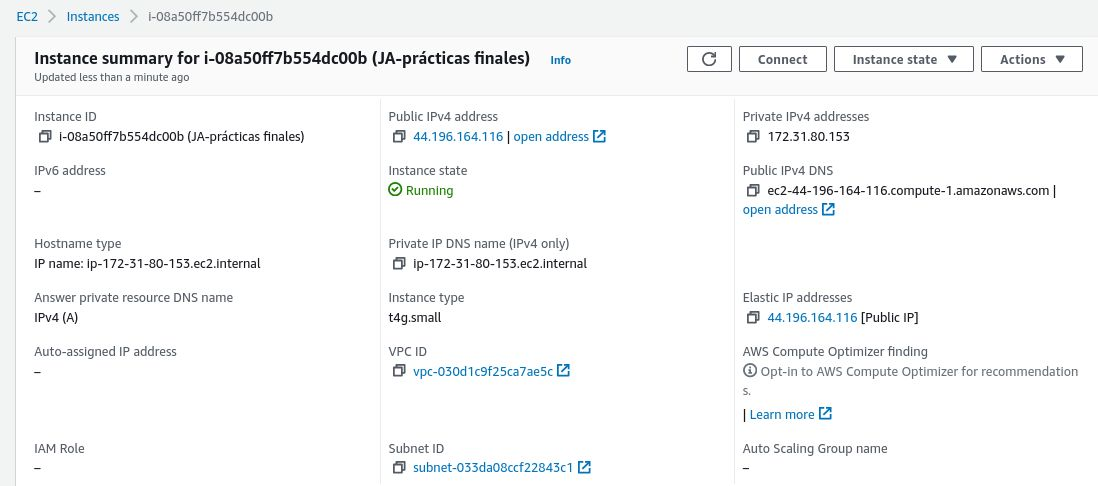
\includegraphics[scale=0.6]{images/broker_aws.jpg}
\end{figure}
 
Los parámetros de conexión son los siguientes:
\begin{itemize}
\item IP estática: 44.196.164.116
\item Puerto: 1883
\end{itemize}


La conexión por el momento no es segura, es decir, sin cifrado SSL y la única seguridad que tiene es que no se permiten usuarios anónimos y se requiere ingresar con usuario y contraseña (tiene que estar registrado).
\begin{figure}[H]
\centering
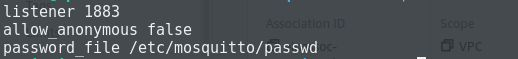
\includegraphics[scale=1]{images/conf_inicial_broker.jpg}
\end{figure}

\subsection*{Pruebas de alimentación con baterías}
Se probó el ESP8266 sin ninguna placa de desarrollo, es decir, solamente el encapsulado. Para eso, se le agregó un regulador, el circuito básico para programarlo y baterías AA para la alimentación.\\\\
Se midió el consumo de corriente sin ningún otro componente y luego con 4 leds de salida, como se muestra a continuación:
	
\begin{figure}[H]
\centering
\includegraphics[scale=0.1]{images/prueba_bateria_1.jpg}
\end{figure}

\begin{figure}[H]
\centering
\includegraphics[scale=0.1]{images/prueba_bateria_2.jpg}
\end{figure}

Lamentablemente el consumo de corriente es muy alto y requeriría un juego de baterías de alta capacidad, haciendo el producto muy voluminoso y costoso, por tanto, no sería atractivo comercialmente. 
\\\\
Por ejemplo, la autonomía con baterías de 3000mAh y un consumo promedio de 75mA sería:

$$t = \frac{3000mAh}{75mA}=40horas$$

Como conclusión, no se van a utilizar baterías para la alimentación. Se va a optar para el ``ESP8266 interruptor'' un transformador y para el ``ESP8266 sensores'' y ``ESP8266 detector'', alimentación por cargador.

\newpage
\section*{Semana, 12 de septiembre - 16 de Septiembre}
Para esta fase se realizó el esquemático de nuestro ESP8266-interruptor en kicad, colocando los footprints de los components que se van a utilizar y se realizó la primera versión de nuestro cliente mqtt web.
\subsection*{Esquemático ESP8266-Interruptor}
\begin{figure}[H]
\centering
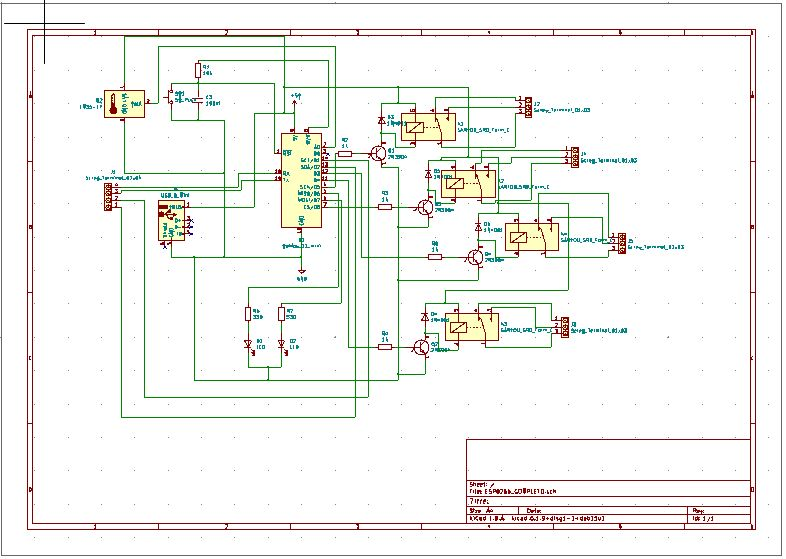
\includegraphics[scale=0.9]{images/esquematico.jpg}
\caption{Esquemático ESP8266-Interruptor}
\end{figure}

Selección de footprints de acuerdo a componentes THT estándar:
\begin{figure}[H]
\centering
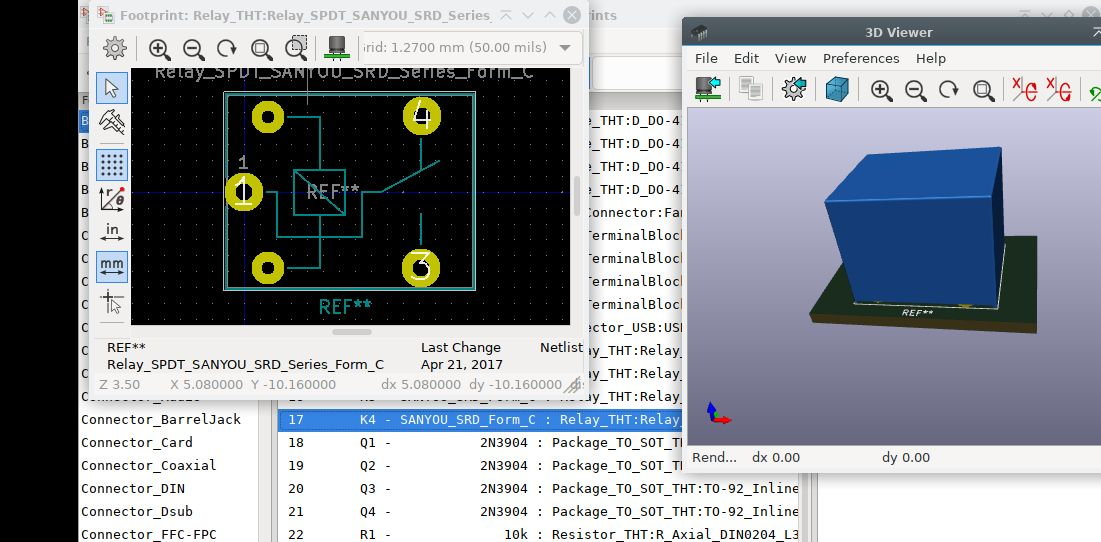
\includegraphics[scale=0.5]{images/footprint1.jpg}
\caption{Footprint relay}
\end{figure}

\begin{figure}[H]
\centering
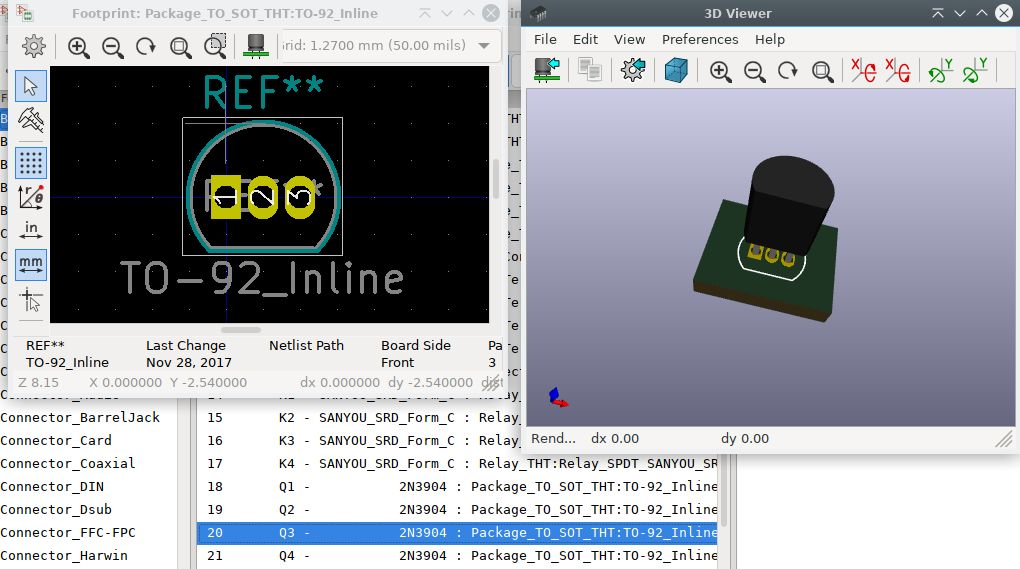
\includegraphics[scale=0.5]{images/footprint2.jpg}
\caption{Footprint transistor 2n3904}
\end{figure}

\pagebreak
También se realizó la primera versión de una aplicación web para comunicarse con nuestros dispositivos mediante WebSockets y MQTT.

\subsection*{Eclipse Paho JavaScript Client}
Paho JavaScript Client es una librería para clientes usando navegadores web en JavaScript, que utiliza WebSockets para conectarse al Broker MQTT.
\\\\
Entre sus principales características tenemos:
\begin{itemize}
\item Soporte para MQTT 3.1
\item Soporte para MQTT 3.1.1
\item Certificados SSL/TLS
\item Reconexión automática
\item Alta disponibilidad
\item Soporte para WebSockets
\end{itemize}

Su instalación consiste en los siguientes pasos:
\begin{enumerate}
\item Copiar todo el código fuente de la librería https://cdnjs.cloudflare.com/ajax/libs/paho-mqtt/1.0.1/mqttws31.js en un archivo JavaScript con el nombre mqttws31.js
\item Hacer referencia de mqttws31.js en la archivo html con \verb@<script src="js/mqttws31.js"></script>@
\end{enumerate}
\subsection*{Bootstrap}
Para darle un buen diseño a la página web y además hacerla responsive, se utiliza Bootstrap 5 y su utilización es la siguiente:
\begin{enumerate}
\item Obtener Bootstrap a través de un CDN (Content Delivery Network): \url{https://cdn.jsdelivr.net/npm/bootstrap@5.2.1/dist/css/bootstrap.min.css}
\item Hacer referencia a Bootstrap en la etiqueta \verb@<head>@ con\\ \verb%<link href="https://cdn.jsdelivr.net/npm/bootstrap@5.2.1/dist/css/bootstrap.min.css"% \\
\verb%rel="stylesheet">%
\end{enumerate}

\subsection*{amCharts 5}
amCharts 5 es una librería JavaScript para la visualización de datos, tiene diferentes tipos de gráficos:
\begin{itemize}
\item X/Y
\begin{itemize}
\item Área
\item Barras y columnas
\item burbujas y dispersión
\item etc.
\end{itemize}
\item Porcentaje
\item mapas geográficos
\item Mucho más
\end{itemize}

Su utilización consiste en agregar referencias a cdns en la etiqueta \verb@<head>@:
\begin{lstlisting}
<script src="https://cdn.amcharts.com/lib/5/index.js"></script>
<script src="https://cdn.amcharts.com/lib/5/xy.js"></script>
<script src="https://cdn.amcharts.com/lib/5/radar.js"></script>
<script src="https://cdn.amcharts.com/lib/5/themes/Animated.js"></script>
\end{lstlisting}

\subsection*{Archivo HTML}
El código en el archito html es:
\begin{lstlisting}
<!DOCTYPE html>
<html lang="en">
<head>
    <meta charset="UTF-8">
    <meta http-equiv="X-UA-Compatible" content="IE=edge">
    <meta name="viewport" content="width=device-width, initial-scale=1.0">
    <title>Domotica Apli1</title>
    <link href="https://cdn.jsdelivr.net/npm/bootstrap@5.2.1/dist/css/bootstrap.min.css"
    rel="stylesheet">
    <link rel="stylesheet" href="css/estilos.css">
    <!--opcion 1-->
    <!--<script src="https://cdnjs.cloudflare.com/ajax/libs/paho-mqtt/1.0.1/mqttws31.js"
    type="text/javascript"></script>-->
    <!--opcion 2-->
    <script src="js/mqttws31.js"></script>
    <script src="https://cdn.amcharts.com/lib/5/index.js"></script>
    <script src="https://cdn.amcharts.com/lib/5/xy.js"></script>
    <script src="https://cdn.amcharts.com/lib/5/radar.js"></script>
    <script src="https://cdn.amcharts.com/lib/5/themes/Animated.js"></script>

</head>
<body>
    <nav class="navbar navbar-expand-sm bg-dark navbar-dark">
        <div class="container-fluid">
          <a class="navbar-brand" href="#">Logo</a>
          <button class="navbar-toggler" type="button" data-bs-toggle="collapse"
          data-bs-target="#collapsibleNavbar">
            <span class="navbar-toggler-icon"></span>
          </button>
          <div class="collapse navbar-collapse" id="collapsibleNavbar">
            <ul class="navbar-nav">
              <li class="nav-item">
                <a class="nav-link" href="#">Link</a>
              </li>
              <li class="nav-item">
                <a class="nav-link" href="#">Link</a>
              </li>
              <li class="nav-item">
                <a class="nav-link" href="#">Link</a>
              </li>  
              <li class="nav-item dropdown">
                <a class="nav-link dropdown-toggle" href="#" 
                role="button" data-bs-toggle="dropdown">Dropdown</a>
                <ul class="dropdown-menu">
                  <li><a class="dropdown-item" href="#">Link</a></li>
                  <li><a class="dropdown-item" href="#">Another link</a></li>
                  <li><a class="dropdown-item" href="#">A third link</a></li>
                </ul>
              </li>
            </ul>
          </div>
        </div>
      </nav>
    <div class="container-fluid">
    <div class="row">
        <div class="col-sm-4 bg-primary text-white">
            <div class="d-grid">
                <button type="button" class="btn btn-primary btn-block"
                onclick="switchGPIO('Led5','ON')">GPIO5 ON</button>
                <button type="button" class="btn btn-primary btn-block"
                onclick="switchGPIO('Led5','OFF')">GPIO5 OFF</button>
            </div>
        </div>
        <div class="col-sm-4 bg-dark text-white">
            <div class="d-grid">
                <button type="button" class="btn btn-dark btn-block"
                onclick="switchGPIO('Led4','ON')">GPIO4 ON</button>
                <button type="button" class="btn btn-dark btn-block"
                onclick="switchGPIO('Led4','OFF')">GPIO4 OFF</button>
            </div>
        </div>
        <div class="col-sm-4 bg-primary text-white">
            <div class="d-grid">
                <button type="button" class="btn btn-primary btn-block"
                onclick="switchGPIO('Led0','ON')">GPIO0 ON</button>
                <button type="button" class="btn btn-primary btn-block"
                onclick="switchGPIO('Led0','OFF')">GPIO0 OFF</button>
            </div>
        </div>
        
    </div>
    <div class="row">
        <div class="col-sm-4 bg-primary text-white">
            <div class="d-grid">
                <button type="button" class="btn btn-primary btn-block"
                onclick="switchGPIO('Led2','ON')">GPIO2 ON</button>
                <button type="button" class="btn btn-primary btn-block"
                onclick="switchGPIO('Led2','OFF')">GPIO2 OFF</button>
            </div>
        </div>
        <div class="col-sm-4 bg-dark text-white">
            <div class="d-grid">
                <button type="button" class="btn btn-dark btn-block"
                onclick="switchGPIO('Led14','ON')">GPIO14 ON</button>
                <button type="button" class="btn btn-dark btn-block"
                onclick="switchGPIO('Led14','OFF')">GPIO14 OFF</button>
            </div>
        </div>
        <div class="col-sm-4 bg-primary text-white">
            <div class="d-grid">
                <button type="button" class="btn btn-primary btn-block"
                onclick="switchGPIO('Led12','ON')">GPIO12 ON</button>
                <button type="button" class="btn btn-primary btn-block"
                onclick="switchGPIO('Led12','OFF')">GPIO12 OFF</button>
            </div>
        </div>
        
    </div>
    <div class="row">
        <div class="col-sm-6">
            <div id="chartdiv"></div>
        </div>
        <div class="col-sm-6">
          <div id="chartdiv2"></div>
      </div>
    </div>

    </div>
       
    <script src="js/iot_mqtt.js"></script>
    <script src="js/graficas.js"></script>

</body>
</html>
\end{lstlisting}

La estructura del la aplicación web queda:
\begin{figure}[H]
\centering
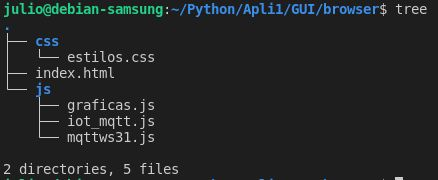
\includegraphics[scale=0.75]{images/estructura.jpg}
\caption{Estructura Página Web}
\end{figure}

Los demás archivos se pueden ver en 
Github: \url{https://github.com/sanic16/Apli1_gui/tree/main/GUI/browser}, donde también está alojado todo el proyecto.

\section*{Semana, 19 de septiembre - 23 de Septiembre}


  

\end{document}